% CHKTEX-FILE 1
% \documentclass[letterpaper,10.5pt,twocolumn]{article}
\documentclass[letterpaper,10.5pt]{article}\usepackage[utf8]{inputenc}
\usepackage[T1]{fontenc}
\usepackage[english,spanish,mexico,es-lcroman]{babel}
% Standard packages
\usepackage{float}
\usepackage{ifthen}
\usepackage{xspace}
\usepackage{amsmath}
\usepackage{xstring}
\usepackage{wrapfig}
\usepackage{booktabs}
\usepackage{csquotes}
\usepackage{fancyhdr}
\usepackage{fancyvrb}
\usepackage{geometry}
\usepackage{graphicx}
\usepackage{lastpage}
\usepackage{listings}
\usepackage{multicol}
\usepackage{multirow}
\usepackage{tabularx}
\usepackage{algorithm}
\usepackage{textgreek}
\usepackage[justification=centering]{subcaption}
\usepackage{algpseudocode}
\usepackage[all]{nowidow}
\usepackage[inline]{enumitem}
\usepackage[usenames,dvipsnames]{xcolor}
% Packages to be loaded later
\usepackage{tikz}
\usepackage{cancel}
\usepackage{tcolorbox}
% Include fullpage images with \includepdf
% \usepackage{pdfpages}
% Referencing
\usepackage{varioref}
\usepackage{hyperref}
\usepackage[noabbrev,nameinlink,spanish]{cleveref}
\usepackage[square, comma, numbers, sort&compress]{natbib}


\newcommand{\lpar}{(}\newcommand{\rpar}{)} %CHKTEX 9
\newcommand{\IIC}{I\textsuperscript{2}C\xspace}
\newcommand{\GND}{\textsc{Gnd}\xspace}
\newcommand{\VCC}{\textsc{Vcc}\xspace}
\newcommand{\VDD}{\textsc{Vdd}\xspace}
\newcommand{\textbi}[1]{\textbf{\textit{#1}}}
\newcommand{\degreesC}[1]{%
	#1\textsuperscript{o}C\xspace{}%
}
\newcommand{\degreesF}[1]{%
	#1\textsuperscript{o}F\xspace{}%
}

% \newcommand{\VCC}{V\textsubscript{CC}\xspace{}}
% \newcommand{\GND}{\textsc{Gnd}\xspace{}}
% CHKTEX-FILE 26
% CHKTEX-FILE 36

\tcbuselibrary{most}
% \tcbuselibrary{listings,breakable}
% \usetikzlibrary{shadings,shadows}
% \usetikzlibrary{decorations.pathmorphing}
% \usetikzlibrary{patterns}
% \usetikzlibrary{spy}
% \usetikzlibrary{arrows.meta}

\newtcolorbox{importantbox}[1]{%
	enhanced,
	colback=red!5!white,%
	colframe=red!75!black,%
	fonttitle=\bfseries,%
	center title,
	title={#1},%
	drop fuzzy shadow
}

\newtcolorbox{marker}[1][]{%
	enhanced,
	before skip=2mm,after skip=3mm,
	boxrule=0.4pt,left=5mm,right=2mm,top=1mm,bottom=1mm,
	colback=yellow!50,
	colframe=yellow!20!black,
	sharp corners,rounded corners=southeast,arc is angular,arc=3mm,
%	underlay={%
%		\path[fill=tcbcolback!80!black] ([yshift=3mm]interior.south east)--++(-0.4,-0.1)--++(0.1,-0.2);
%		\path[draw=tcbcolframe,shorten <=-0.05mm,shorten >=-0.05mm] ([yshift=3mm]interior.south east)--++(-0.4,-0.1)--++(0.1,-0.2);
%		\path[fill=yellow!50!black,draw=none] (interior.south west) rectangle node[white]{\Huge\bfseries !} ([xshift=4mm]interior.north west);
%	},
	drop fuzzy shadow,#1
}

%CHKTEX-FILE 1
%CHKTEX-FILE 7
%CHKTEX-FILE 9
% Default fixed font does not support bold face
\DeclareFixedFont{\ttb}{T1}{txtt}{bx}{n}{8} % for bold
\DeclareFixedFont{\ttm}{T1}{txtt}{m}{n}{8}  % for normal

% Custom colors
\usepackage{color}
\definecolor{keywordsColor}{rgb}{0,0,0.5}
\definecolor{customColor}{rgb}{0.6,0,0}
\definecolor{stringColor}{rgb}{0,0.5,0}

% Code highlighting python
\renewcommand{\ttdefault}{pcr}
\lstset{
	language=Python,                              % the language of the code (can be overrided per snippet)
	backgroundcolor=\color{white},                % choose the background color
	basicstyle=\footnotesize\ttfamily,            % the size of the fonts that are used for the code
	breakatwhitespace=false,                      % sets if automatic breaks should only happen at whitespace
	breaklines=true,                              % sets automatic line breaking
	captionpos=t,                                 % sets the caption-position to bottom
	commentstyle=\color{gray},                    % comment style
	deletekeywords={},                            % if you want to delete keywords from the given language
%	escapeinside={\%*}{*)},                       % if you want to add LaTeX within your code
	extendedchars=true,                           % lets you use non-ASCII characters; for 8-bits encodings only, does not work with UTF-8
	frame=tb,                                     % adds a frame around the code
	keepspaces=true,                              % keeps spaces in text, useful for keeping indentation of code (possibly needs columns=flexible)
	keywordstyle=\color{keywordsColor}\bfseries,  % keyword style
	numbers=left,                                 % where to put the line-numbers; possible values are (none, left, right)
	numbersep=5pt,                                % how far the line-numbers are from the code
	numberstyle=\tiny\color{gray},                % the style that is used for the line-numbers
	rulecolor=\color{black},                      % if not set, the frame-color may be changed on line-breaks within not-black text (e.g. comments (green here))
	showspaces=false,                             % show spaces everywhere adding particular underscores; it overrides 'showstringspaces'
	showstringspaces=false,                       % underline spaces within strings only
	showtabs=false,                               % show tabs within strings adding particular underscores
	stepnumber=1,                                 % the step between two line-numbers. If it's 1, each line will be numbered
	stringstyle=\color{stringColor},              % string literal style
	tabsize=2,                                    % sets default tabsize to 2 spaces
	title=\lstname,                               % show the filename of files included with \lstinputlisting; also try caption instead of title
	columns=fixed,                                % Using fixed column width (for e.g. nice alignment)
	otherkeywords={self},                         % if you want to add more keywords to the set
	emphstyle=\color{customColor}\bfseries,       % Custom highlighting style
	emph={__init__,__main__,True,False,None},     % Custom highlighting keywords
	xleftmargin=1cm,                              % Left margin
	xrightmargin=1cm,                             % Right margin
	% Unicode compatibility
	inputencoding=utf8,
	literate={%
	            {Á}{{\'a}}1 {É}{{\'E}}1 {Í}{{\'I}}1 {Ó}{{\'O}}1 {Ú}{{\'U}}1%
	            {á}{{\'a}}1 {é}{{\'e}}1 {í}{{\'i}}1 {ó}{{\'o}}1 {ú}{{\'u}}1%
	            {À}{{\`A}}1 {È}{{\'E}}1 {Ì}{{\`I}}1 {Ò}{{\`O}}1 {Ù}{{\`U}}1%
	            {à}{{\`a}}1 {è}{{\`e}}1 {ì}{{\`i}}1 {ò}{{\`o}}1 {ù}{{\`u}}1%
	            {Ä}{{\"A}}1 {Ë}{{\"E}}1 {Ï}{{\"I}}1 {Ö}{{\"O}}1 {Ü}{{\"U}}1%
	            {ä}{{\"a}}1 {ë}{{\"e}}1 {ï}{{\"i}}1 {ö}{{\"o}}1 {ü}{{\"u}}1%
	            {Â}{{\^A}}1 {Ê}{{\^E}}1 {Î}{{\^I}}1 {Ô}{{\^O}}1 {Û}{{\^U}}1%
	            {â}{{\^a}}1 {ê}{{\^e}}1 {î}{{\^i}}1 {ô}{{\^o}}1 {û}{{\^u}}1% CHKTEX 19
	            {Ã}{{\~a}}1 {Ẽ}{{\~E}}1 {Ĩ}{{\~I}}1 {Õ}{{\~O}}1 {Ũ}{{\~U}}1 {Ñ}{{\~N}}1%
	            {ã}{{\~a}}1 {ẽ}{{\~e}}1 {ĩ}{{\~i}}1 {õ}{{\~o}}1 {ũ}{{\~u}}1 {ñ}{{\~n}}1%
	            {œ}{{\oe}}1 {Œ}{{\OE}}1 {æ}{{\ae}}1 {Æ}{{\AE}}1 {ß}{{\ss}}1%
	            {ç}{{\c c}}1 {Ç}{{\c C}}1 {ø}{{\o}}1 {å}{{\r a}}1 {Å}{{\r A}}1%
	            {€}{{\EUR}}1 {£}{{\pounds}}1 {×}{{\(\times\)}}1% CHKTEX 21
	            {°}{{\textsuperscript{o}}}1%
	            {¹}{{\textsuperscript{1}}}1%
	            {²}{{\textsuperscript{2}}}1%
	            {³}{{\textsuperscript{3}}}1%
	            {⁴}{{\textsuperscript{4}}}1% CHKTEX 19
	            {⁵}{{\textsuperscript{5}}}1% CHKTEX 19
	            {⁶}{{\textsuperscript{6}}}1% CHKTEX 19
	            {⁷}{{\textsuperscript{7}}}1% CHKTEX 19
	            {⁸}{{\textsuperscript{8}}}1% CHKTEX 19
	            {⁹}{{\textsuperscript{9}}}1% CHKTEX 19
	            {⁰}{{\textsuperscript{0}}}1% CHKTEX 19
%	            {A}{{\textAlpha}}1
	            {α}{{\textalpha}}1%
%	            {B}{{\textBeta}}1
	            {β}{{\textbeta}}1%
	            {Γ}{{\textGamma}}1
	            {γ}{{\textgamma}}1%
	            {Δ}{{\textDelta}}1
	            {δ}{{\textdelta}}1% CHKTEX 19
%	            {E}{{\textEpsilon}}1
	            {ϵ}{{\textepsilon}}1%
%	            {Z}{{\textZeta}}1
	            {ζ}{{\textzeta}}1%
%	            {H}{{\textEta}}1
	            {η}{{\texteta}}1%
	            {Θ}{{\textTheta}}1
	            {θ}{{\texttheta}}1%
%	            {I}{{\textIota}}1
	            {ι}{{\textiota}}1%
%	            {K}{{\textKappa}}1
	            {κ}{{\textkappa}}1%
	            {Λ}{{\textLambda}}1
	            {λ}{{\textlambda}}1%
%	            {M}{{\textMu}}1
	            {μ}{{\textmu}}1%
%	            {N}{{\textNu}}1
	            {ν}{{\textnu}}1%
	            {Ξ}{{\textXi}}1
	            {ξ}{{\textxi}}1%
%	            {O}{{\textOmikron}}1
%	            {o}{{\textomikron}}1%
	            {Π}{{\textPi}}1
	            {π}{{\textpi}}1%
%	            {P}{{\textRho}}1
	            {ρ}{{\textrho}}1%
	            {Σ}{{\textSigma}}1
	            {σ}{{\textsigma}}1%
%	            {T}{{\textTau}}1
	            {τ}{{\texttau}}1%
	            {ϒ}{{\textUpsilon}}1
	            {υ}{{\textupsilon}}1%
	            {Φ}{{\textPhi}}1
	            {ϕ}{{\textphi}}1%
%	            {X}{{\textChi}}1
	            {χ}{{\textchi}}1%
	            {Ψ}{{\textPsi}}1
	            {ψ}{{\textpsi}}1%
	            {Ω}{{\textOmega}}1
	            {ω}{{\textomega}}1%
	            {ζ}{{\varsigma}}1%
%	            {}{{\straightphi}}1%
%	            {}{{\scripttheta}}1%
%	            {}{{\straighttheta}}1%
%	            {}{{\straightepsilon}}1%
	         },
}

\lstdefinestyle{c_with_comments}%
{
	language     = c,
	morecomment  = [l]{//},
	morecomment  = [s]{/*}{*/},
	breaklines,
}

\lstdefinestyle{c_without_comments}%
{
	style        = c_with_comments,
	% numbers      = none,
	% keepspaces   = false,
	morecomment  = [l][\nullfont]{//},
	morecomment  = [is]{//}{\^^M},
	morecomment  = [is]{/*}{*/},
}

\lstdefinelanguage{conf}
{
	basicstyle=\ttfamily\small,
	columns=fullflexible,
	morecomment=[s][\color{Orchid}\bfseries]{[}{]},
	morecomment=[l]{\#},
	morecomment=[l]{;},
	commentstyle=\color{gray}\ttfamily,
	% morekeywords={},
	% otherkeywords={=,:},
	% keywordstyle={\color{Green}\bfseries}
}

% \captionsetup[lstlisting]{font={small,tt}}
\captionsetup[lstlisting]{%
	font={small},
}



\DefineVerbatimEnvironment{Verbatim}{Verbatim}{%
	fontsize=\footnotesize,%
	frame=leftline,%
	framesep=2em,    % separation between frame and text
}

\RecustomVerbatimCommand{\VerbatimInput}{VerbatimInput}{%
	fontsize=\footnotesize,
%	frame=lines,            % top and bottom rule only
	frame=leftline,         % left rule only
	numbers=left,           % Line numbers on the left
	numbersep=0.25em,       % Gap between numbers and verbatim lines
	xleftmargin=4em,        % Indentation to add at the start of each line
	xrightmargin=4em,       % Right margin to add after each line
	framesep=0.5em,         % separation between frame and text
	rulecolor=\color{Gray}, % Color of the lines
	labelposition=topline,  %
	samepage=false,         % When true, prevents verbatim environment from
	                        % being broken between pages
%	commandchars=\|\(\),    % escape character and argument delimiters for
	                        % commands within the verbatim
%	commentchar=*           % comment character
}


\hypersetup{
	hidelinks,
	colorlinks=true,
	linkcolor=Blue,
	filecolor=OliveGreen,
	urlcolor=RoyalPurple,
	pdfauthor={Mauricio Matamoros},
%	pdftitle={Práctica 0X – Fundamentos de Sistemas Embebidos},
% 	pdfsubject={The Subject},
% 	pdfkeywords={Some Keywords},
% 	pdfproducer={Latex with hyperref, or other system},
% 	pdfcreator={pdflatex, or other tool}
}

\captionsetup{%
	font=small
}

\geometry{%
	margin=2cm,
	% top=3cm,
	bottom=3cm,
	% left=2cm,
	% right=2cm,
	% inner=2cm,
	% outer=2cm,
	% headheight=,
	% footsep=,
	% footskip=,
}

\pagestyle{fancy}
\renewcommand{\headrulewidth}{0.0pt}
\lhead{}
\chead{}
\rhead{}
\lfoot{}
\cfoot{}
\rfoot{Página~\thepage~de~\pageref{LastPage}}

\crefname{table}{tabla}{tablas}
\Crefname{table}{Tabla}{Tablas}
\crefname{section}{sección}{secciones}
\Crefname{section}{Sección}{Secciones}
\crefname{subsection}{subsección}{subsecciones}
\Crefname{subsection}{Subsección}{Subsecciones}
\crefname{listing}{código de ejemplo}{códigos de ejemplo}
\Crefname{listing}{Código de Ejemplo}{Códigos de Ejemplo}
\renewcommand*{\lstlistingname}{Código ejemplo}


\hypersetup{
	hidelinks,
	pdfauthor={Mauricio Matamoros},
	pdftitle={Programa 01 – Fundamentos de Sistemas Embebidos},
% 	pdfsubject={The Subject},
% 	pdfkeywords={Some Keywords},
% 	pdfproducer={Latex with hyperref, or other system},
% 	pdfcreator={pdflatex, or other tool}
}

\author{\footnotesize Autor: José Mauricio Matamoros de Maria y Campos}
\title{Programa 1:\\Puerto GPIO de la Raspberry Pi en simulador\\
{\large Fundamentos de Sistemas Embebidos}}
\date{}


% Document body
\begin{document}
\maketitle

\section{Objetivo}%
\label{sec:objective}
El alumno se familiarizará con el puerto GPIO de la Raspberry Pi (simulado), configurándo varios pines como salidas digitales para el control de leds y circuitos de lógica TTL.%

\section{Material}%
\label{sec:material}
Ninguno


% Se controlará el encendido y apagado de LEDS usando la Raspberry Pi

\section{Instrucciones}%
\label{sec:instructions}
\begin{enumerate}[noitemsep]
	\item Descargue y pruebe la tarjeta simuladora siguiendo los pasos de la \cref{sec:step1}
	\item Realice los programas de las \cref{sec:step2,sec:step3,sec:step4}
	\item Analice los programas de las \cref{sec:step2,sec:step3,sec:step4}, realice los experimentos propuestos en la \cref{sec:experiments} y con los resultados obtenidos responda el cuestionario de la \cref{sec:questionnaire}.
\end{enumerate}

% %% %%%%%%%%%%%%%%%%%%%%%%%%%%%%%%%%%%%%%%%%%%%%%%%%%%%%%%%%%%%%%%%%%%
%
% Step 1
%
% %% %%%%%%%%%%%%%%%%%%%%%%%%%%%%%%%%%%%%%%%%%%%%%%%%%%%%%%%%%%%%%%%%%%
\subsection{Paso 1: Configuración del Simulador}%
\label{sec:step1}

Descargue el simulador de \url{https://github.com/kyordhel/RPiVirtualBoard} ejecutando la siguiente línea de comandos:

\begin{Verbatim}[fontsize=\footnotesize]
git clone https://github.com/kyordhel/RPiVirtualBoard.git
cd RPiVirtualBoard
\end{Verbatim}

A continuación instale todas las dependencias requeridas por el simulador usando \emph{pip}:

\begin{Verbatim}[fontsize=\footnotesize]
sudo apt install python3-tk
pip install --user -r requirements.txt
\end{Verbatim}

Finalmente, pruebe el simulador ejecutando la siguiente línea:

\begin{Verbatim}[fontsize=\footnotesize]
./blink.py
\end{Verbatim}

O bien, si desea mantener el simulador conmo un proyecto aislado y cuenta con la utilería \emph{pipenv}\footnotemark{} para tal propósito, después de clonar el proyecto basta con ejecutar:

\begin{Verbatim}[fontsize=\footnotesize]
pipenv run python blink.py
\end{Verbatim}

Si la configuración es correcta, verá una ventana similar a la de la \Cref{fig:simboard} con uno de los leds virtuales parpadeando.
Este simulador implementa el circuito mostrado en la \Cref{fig:wiring-diagram}

\begin{figure}[H]
	\centering%
	\begin{subfigure}{0.49\textwidth}
		\centering%
		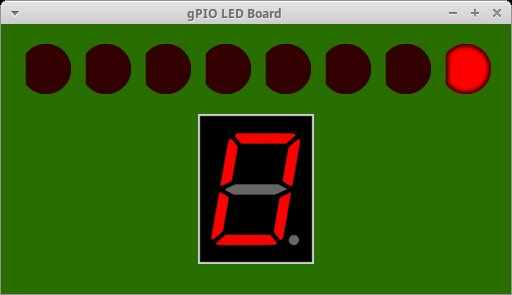
\includegraphics[width=0.9\textwidth,height=8cm,keepaspectratio]{img/simboard.jpg} %CHKTEX 8
		\caption{Simulador de tarjeta con leds para la GPIO de la Raspberry Pi}
		\label{fig:simboard} %CHKTEX 24
	\end{subfigure}
	\hfill
	\begin{subfigure}{0.49\textwidth}
		\centering%
		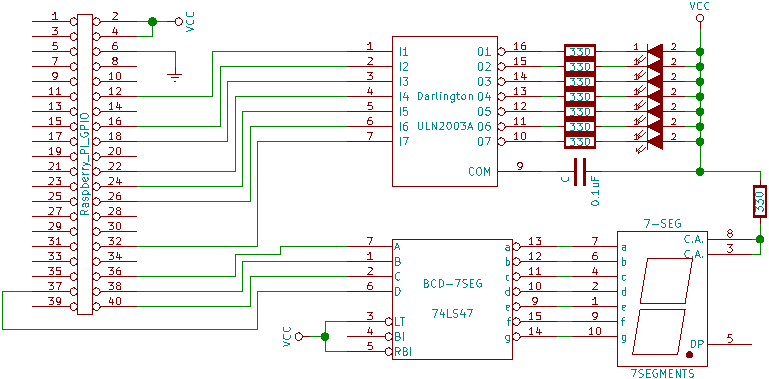
\includegraphics[width=0.9\columnwidth,height=8cm,keepaspectratio]{img/diagram.pdf} %CHKTEX 8
		\caption{Circuito implementado en el simulador}
		\label{fig:wiring-diagram} %CHKTEX 24
	\end{subfigure}
	\caption{Simulador y circuito implementado}
	\label{fig:sim} %CHKTEX 24
\end{figure}

\footnotetext{\emph{pipenv} es una herramienta que facilita la creación y administración de entornos virtuales en cualquier proyecto escritos en Python, llevando un control riguroso de los paquetes de los que depende dicho proyecto. Se puede instalar fácilmente con la línea \texttt{pip install --user pipenv}}



% %% %%%%%%%%%%%%%%%%%%%%%%%%%%%%%%%%%%%%%%%%%%%%%%%%%%%%%%%%%%%%%%%%%%
%
% Step 2
%
% %% %%%%%%%%%%%%%%%%%%%%%%%%%%%%%%%%%%%%%%%%%%%%%%%%%%%%%%%%%%%%%%%%%%
\subsection{Paso 2: Led parpadeante}%
\label{sec:step2}
El código mostrado en \Cref{src:blink} muestra cómo se haría parpadear un LED mediante tiempos de espera o \emph{sleeps} utilizando la Raspberry Pi.

\smallskip
\lstinputlisting[%
	language=Python,
	linerange={18-40}, % chktex 8
	caption={\texttt{blink.py}},
	label={src:blink}
]{src/blink.py}
\smallskip

Estudie el código y véalo en funcionamiento, ejecutándolo de la siguiente manera:
\begin{Verbatim}[fontsize=\footnotesize]
./blink.py
\end{Verbatim}

% %% %%%%%%%%%%%%%%%%%%%%%%%%%%%%%%%%%%%%%%%%%%%%%%%%%%%%%%%%%%%%%%%%%%
%
% Step 3
%
% %% %%%%%%%%%%%%%%%%%%%%%%%%%%%%%%%%%%%%%%%%%%%%%%%%%%%%%%%%%%%%%%%%%%
\subsection{Paso 3: Led parpadeante con PWM}%
\label{sec:step3}
En lugar de utilizar tiempos de espera (mismos que consumen tiempo de procesamiento y energía), es posible hacer parpadear el led de manera mucho más precisa y rápida utilizando uno de los moduladores de ancho de pulso (en inglés \emph{Pulse Width Modulation} o \emph{PWM}) por hardware que incorpora la Raspberry Pi.

El código mostrado en \Cref{src:pwm} muestra cómo se haría parpadear un LED mediante \emph{PWM} utilizando la Raspberry Pi.

\smallskip
\lstinputlisting[%
	language=Python,
	linerange={18-54}, % chktex 8
	caption={\texttt{pwm.py}},
	label={src:pwm}
]{src/pwm.py}
\smallskip

Estudie el código y véalo en funcionamiento, ejecutándolo de la siguiente manera:
\begin{Verbatim}[fontsize=\footnotesize]
./pwm.py
\end{Verbatim}


% %% %%%%%%%%%%%%%%%%%%%%%%%%%%%%%%%%%%%%%%%%%%%%%%%%%%%%%%%%%%%%%%%%%%
%
% Step 5
%
% %% %%%%%%%%%%%%%%%%%%%%%%%%%%%%%%%%%%%%%%%%%%%%%%%%%%%%%%%%%%%%%%%%%%
\subsection{Paso 4: Display de siete segmentos}%
\label{sec:step4}
El código mostrado en \Cref{src:bcd} muestra cómo se operaría un display de siete segmentos mediante una controladora TTL 74LS47 utilizando la Raspberry Pi.

\smallskip
\lstinputlisting[%
	language=Python,
	linerange={19-51}, % chktex 8
	caption={\texttt{bcd.py}},
	label={src:bcd}
]{src/bcd.py}
\smallskip

Estudie el código y véalo en funcionamiento, ejecutándolo de la siguiente manera:
\begin{Verbatim}[fontsize=\footnotesize]
./bcd.py
\end{Verbatim}

% %% %%%%%%%%%%%%%%%%%%%%%%%%%%%%%%%%%%%%%%%%%%%%%%%%%%%%%%%%%%%%%%%%%%
%
% Programs
%
% %% %%%%%%%%%%%%%%%%%%%%%%%%%%%%%%%%%%%%%%%%%%%%%%%%%%%%%%%%%%%%%%%%%%
\section{Programas}%
\label{sec:programs}

Genere un conjunto de 5 programas que resuelvan los siguientes problemas.

\begin{enumerate}
	\item{} [1pt] Modifique el código de la \cref{sec:step2} para todos los leds de la fila parpadeen.
	Nombre el archivo de código fuente \texttt{blink8.py}

	\item{} [1pt] Modifique el código de las \cref{sec:step2,sec:step3} para que los leds de la fila enciendan de manera continua en una marquesina de izquierda a derecha.
	Nombre el archivo de código fuente \texttt{marquee.py}

	\item{} [2pt] Modifique el código de la \cref{sec:step2} para que ocho leds parpadeen en el simulador en línea \url{https://create.withcode.uk/python/A3}.
	Nombre el archivo de código fuente \texttt{osblink8.py}
	Proporcione un video (captura de pantalla) con nombre \texttt{osblink8.mp4}, sin audio y con \emph{codec} h.264 a 15fps como evidencia.

	\item{} [2pt] Modifique el código de las \cref{sec:step2,sec:step3} para que 8 leds en la misma fila del simulador en línea el simulador en línea \url{https://create.withcode.uk/python/A3} enciendan de manera continua en una marquesina de izquierda a derecha.
	Nombre el archivo de código fuente \texttt{osmarquee.py}
	Proporcione un video (captura de pantalla) con nombre \texttt{osmarquee.mp4}, sin audio y con \emph{codec} h.264 a 15fps como evidencia.

	\item{} [2pt] Modifique el código de las \cref{sec:step2,sec:step3,sec:step4}, para que los últimos 4 leds de la derecha muestren el código BCD enviado al display de 7 segmentos.
	Nombre el archivo de código fuente \texttt{bcd.py}
\end{enumerate}

\section{Especificaciones técnicas de los programas}%
\label{sec:programs-specs}
\begin{itemize}[noitemsep]
	\item No utilice paquetes adicionales.
	\item El código deberá ser ejecutable con Python versión 3.5 o posterior.
	\item Todos los programas deberán comenzar con la línea de intérprete o \emph{she-bang} correspondiente
	\item Todos los programas deberán tener el nombre del autor de la forma:

\begin{lstlisting}[language=python]
# Author: Nombre del Alumno
\end{lstlisting}

	\item Incluya sólo los videos, el cuestionario, y el código fuente de los programas \textbi{sin librerías ni paquetes}.
	\item Los archivos de código python deberán estar en raíz \texttt{./}.
	\item Los videos-evidencia deberán estar en el subdirectorio \texttt{./vid/}.
	\item Los videos-evidencia deberán durar no más de 60 segundos, incluir sólo la ventana del simulador y contar únicamente con \emph{stream} de video comprimido con \emph{codec} h.264 a \(15fps\) con una resolución máxima de \(1280 \times 720\) y con un tamaño máximo de 3MB por archivo (velocidad de datos aproximada de \(1500kbps\))\footnote{\texttt{ffmpeg -i input -an -vf scale=-1:720 -c:v libx264 -crf 28 -r 15 -preset veryslow hicm\_osblink8.mp4}}.
	\item Anexe el cuestionario en formato \emph{pdf} bajo \texttt{./doc/} como \texttt{questionnaire.pdf}.
	\item Los nombres de todos los archivos proporcionados deberán llevar un prefijo \(p\) de 5 caracteres, tales que:
	\begin{itemize}[noitemsep]
		\item \textbf{\(p[0]\)} Primera letra del apellido paterno del alumno excluyendo preposiciones.
		\item \textbf{\(p[1]\)} Segunda letra del apellido paterno del alumno excluyendo preposiciones.
		\item \textbf{\(p[2]\)} Primera letra del apellido materno del alumno excluyendo preposiciones.
		\item \textbf{\(p[3]\)} Primera letra del primer nombre del alumno o X en caso de nombres compuestos principiantes por J, J., José, Ma., Ma o María.
		\item \textbf{\(p[4]\)} Guión bajo (caracter ASCII 95).
		\item Toda Ñ se reemplaza con una X
	\end{itemize}
	Es decir, las primeras 4 letras de su \href{http://www.renapo.gob.mx/RENAPOPortal/docs/InstructivoParaLaCurp.pdf}{RFC o CURP} seguidas de un guión bajo.
	Así, el cuestionario de Miguel Hidalgo y Costilla quedaría almacenado como \texttt{./doc/hicm\_questionnaire.pdf}.
	\item El conjunto de programas, videos y el questionario deberá estar empaquetado en un archivo comprimido de nombre \texttt{[prefijo]\_p01}, por ejemplo \texttt{hicm\_p01.zip}.
	Los formatos aceptables son \emph{7z}, \emph{rar}, \emph{tar.bz2}, \emph{tar.gz} y \emph{zip}.
\end{itemize}


	% \footnotetext{Archivo de video sin \emph{stream} de audio. Utilice el \emph{codec} h264}}

% %% %%%%%%%%%%%%%%%%%%%%%%%%%%%%%%%%%%%%%%%%%%%%%%%%%%%%%%%%%%%%%%%%%%
%
% Questionnaire
%
% %% %%%%%%%%%%%%%%%%%%%%%%%%%%%%%%%%%%%%%%%%%%%%%%%%%%%%%%%%%%%%%%%%%%
\section{Cuestionario}%
\label{sec:questionnaire}
\begin{enumerate}
	\item{} [2pt] Investigue el efecto que se produciría al regular el tiempo de encendido de un LED mediante la modulación del ciclo de trabajo del PWM en alta frecuencia (ej.~1kHz) y explique por qué no es posible observar este efecto en los simuladores.
\end{enumerate}

\end{document}
